\chapter{Learning-Based Recognition of Human-Grasped Objects}
\label{chapter:learning}

This chapter covers the development of machine learning models to recognize human-grasped objects. In particular, \autoref{section:proposal_framework} formulates the problem with detail and describes the evaluation metrics. \autoref{section:data_representation} details the data collecting and the dataset preprocessing and splitting. \autoref{section:cnn_classifier} and \autoref{section:transformer_classifier} describe the implementation of the \acs{cnn} and Transformer models respectively and their results. \autoref{section:comparative_analysis} compares the results of both models in different cases. \autoref{section:human_intention_prediction} delves into a possible implementation of a real-time implementation of anticipation along with possible limitations and solutions. \autoref{section:learning_final_remarks} provides the final remarks about the models' performance.

\section{Proposal Framework}
\label{section:proposal_framework}

\subsection{Approach}

% The adopted solution  focuses on detecting and tracking the hand and finger keypoints from visual data. 
This dissertation proposes a learning-based framework to enable an assistive robot to recognize the object grasped by the human operator. As illustrated in \autoref{fig:LearningFramework}, the proposed framework combines the strengths of MediaPipe in detecting hand landmarks in a RGB image with a deep multi-class classifier that predicts the object based on the configuration of the user’s hand after grasping it. Accordingly, the developed object recognition system operates based on different principles, including the sensing device, the tracking method, and the machine learning approaches. From the point of view of the application in industrial settings, the proposed system has two strengths when compared to the use of data-gloves or electromagnetic motion capture systems. First, the simplicity of installation is associated with a much less complex and costly setup. Second, the non-intrusiveness of the required setup is a valuable factor in accelerating the acceptance of these technologies by humans in carrying out collaborative tasks (a process also referred to as "user adoption"). In contrast, vision-based hand tracking is affected by occlusions, changes in light conditions, and cluttered backgrounds. Furthermore, these problems are difficult to overcome with deep-learning techniques given the data dependency and generalization problems against hands, objects, and lighting conditions outside the training sets. Overall, this paper contributes to advances in understanding the opportunities and limitations of using this novel approach for the recognition of human-grasped objects.

\begin{figure}[ht]
    \centering
    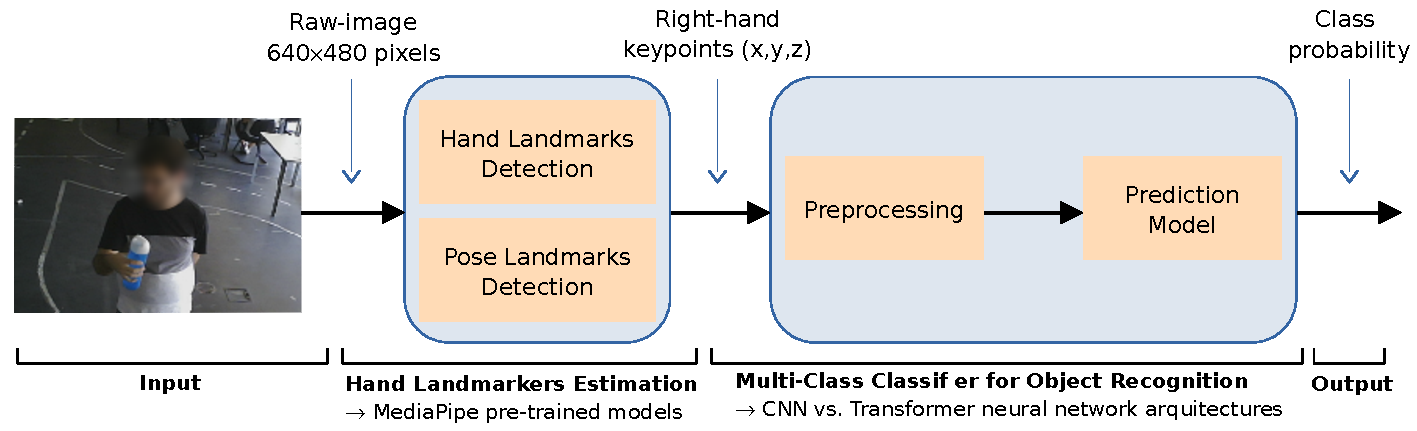
\includegraphics[width=1\columnwidth]{figs/LearningFrameworkB.pdf}
    \caption{The proposed learning-based framework for object recognition based on the hand keypoints.}
    \label{fig:LearningFramework}
\end{figure}

The output of the pre-trained model provides the $(x,y,z)$ coordinates of landmarks for each detected hand. The $(x,y)$ coordinates represent the horizontal and vertical positions of the landmark on the image plane, while the $z$-coordinate represents an estimate of the relative depth with respect to the wrist reference \cite{Amprimo2023}. This work focuses on tracking the right hand by combining the Hand Landmark detection and the Pose Landmark Detection pre-trained models. This strategy proved to be useful to enhance the reliability of the process of extracting the coordinates of the right-hand keypoints from each frame.

The multi-class classifier for object recognition faces several challenges. First, there is limited information about the three-dimensional configuration of the hand, namely if the hand configurations involve overlapping fingers or positions close to each other in the image plane. Consequently, the $z$-coordinate (relative depth) revealed to be a critical element for discriminating complex hand configurations. Second, the coordinates provided by MediaPipe can vary in scale and rotation depending on the hand’s distance from the camera and the hand’s orientation in the image, adding complexity to the task. For these reasons, a deep learning model able to learn complex features directly from the MediaPipe coordinates will be explored and evaluated with a view to its generalization ability in different scenarios and for various users. 

The learning problem involves a mapping between two spaces $f(X,\theta): X \rightarrow Y$, where $X \in \mathbb{R}^{3\times21}$ is the set of possible spatial coordinates of the hand keypoints, $Y \in \mathbb{R}^{M}$ is the set of possible $M$ output classes, and $\theta$ the model parameters. Let $D = \{(x_1,y_1),\cdots,(x_n,y_n)\}$ be a training dataset of $n$ examples where $x_i \in X$ is an input and $y_i \in Y$ is the corresponding ground truth class label. 
Given a new instance $x_{new}$, the task is to predict its corresponding object class $y_{pred}$, such that:
\begin{equation}
y_{pred} = f(x_{new})\text{.}
\end{equation}

The model aims to minimize a chosen loss function $L$ that quantifies the dissimilarity between the predicted class $y_{pred}$ and the ground truth class $y_i$. Formally, the training process seeks to find the optimal parameters $\hat{\theta}$ of the mapping function $f$ by solving the following optimization problem:
\begin{equation}\label{eq:optimaltheta}
\hat{\theta} = \mathop{\mathrm{argmin}}_{\theta}\frac{1}{n} \sum_{i=1}^{n} L\left(f_{\theta}(x_i),y_i\right)\text{,}
\end{equation}
%
where $f_{\theta}(x_i)$ is the predicted class label for sample $x_i$ using the model with parameters $\theta$, and $L$ is a suitable loss function. Upon successful training, the model $f$ can be used for predicting the object class $y_{pred}$ for new instances of hand keypoints.

\subsection{Evaluation Metrics}

To properly ascertain the performance and generalization capability of deep learning models, metrics must be employed. Accuracy is one of the most widely used metrics in the realm of deep learning, representing the proportion of correctly classified examples among all samples in the dataset, calculated as follows: \begin{equation}ACC=\frac{Number\ of\ Correct\ Predictions}{Total\ Number\ of\ Predictions}\text{ .}\label{eq:acc}\end{equation}

Although accuracy clearly assesses the model's performance, it may not be recommended in some situations, like when working with an imbalanced dataset. Therefore other metrics should be used, such as:
\begin{itemize}
    \item True Positive (TP) - instances correctly classified as positive;
    \item True Negative (TN) - instances correctly classified as negative;
    \item False Positive (FP) - instances incorrectly classified as positive;
    \item False Negative (FN) - instances incorrectly classified as negative;
    \item Positive Predictive Value (PPV) or Precision, which is the percentage of instances correctly classified as positive relative to all instances classified as positive: \begin{equation}PPV=\frac{TP}{TP+FP}\text{ ;}\label{eq:ppv}\end{equation}
    \item True Positive Rate (TPR) or Recall, which is the percentage of positive instances that are classified as positive: \begin{equation}TPR=\frac{TP}{TP+FN}\text{ ;}\label{eq:tpr}\end{equation}
    \item F1-Score, which is the harmonic mean between the precision and the recall: \begin{equation}TPR=2\frac{PPV \times TPR}{PPV+TPR}=\frac{2TP}{2TP+FP+FN}\text{ .}\label{eq:f1-score}\end{equation}
\end{itemize}

Precision is a relevant metric to use when the aim is to minimize false positives, while Recall is relevant to minimize false negatives. F1-Score includes the two of them, with both false positives and false negatives influencing the result.

In a multi-class classification problem, such as the one in this work, these metrics are obtained separately for each class and then averaged across all classes to obtain a final metric.

In addition to the previous metrics, a Confusion Matrix can be used to visually represent the model's performance in a tabular way. Each entry $i,j$ contains the number of instances from the class $i$ that are classified as belonging to the class $j$ (e.g., \autoref{fig:non-norm_conf_matrix}). A confusion matrix can also undergo normalization by dividing each entry by the sum of its row so that each entry provides ratios instead (e.g., \autoref{fig:norm_conf_matrix}).

\begin{figure}[ht]
    \centering
    \begin{subfigure}[b]{0.35\textwidth}
        {\fontsize{10}{12}\selectfont\includesvg[width=\textwidth]{figs/conf_matrix_example2.svg}}
        \caption{}
        \label{fig:non-norm_conf_matrix}
    \end{subfigure} \ \
    \begin{subfigure}[b]{0.35\textwidth}
        {\fontsize{10}{12}\selectfont\includesvg[width=\textwidth]{figs/conf_matrix_example.svg}}
        \caption{}
        \label{fig:norm_conf_matrix}
    \end{subfigure}
    \caption[Confusion matrices examples: non-normalized and normalized.]{Confusion matrices examples: (a) non-normalized and (b) normalized.}
    \label{fig:conf_matrix_examples}
\end{figure}

\section{Data Representation}
\label{section:data_representation}

The four objects selected for this study are all "graspable", i.e., more or less rigid. They include a cylindrical water bottle, a Rubik’s cube, a flat and thick smartphone, and a small and sharp screwdriver (\autoref{fig:GraspedObjects}). Given the differences in shape, size, and/or weight, the goal is to discriminate these four objects based on the configuration adopted by the hand while interacting with them. This section will start by validating the MediaPipe framework given the fact that it is an external tool and then it will detail the dataset acquisition, the data pre-processing, and the data splitting. 

\begin{figure}[ht]
\captionsetup{width=0.6\textwidth}
\centering
\adjincludegraphics[width=0.6\textwidth, trim={{0} {0.05\height} {0} {0.1\height}}, clip]{figs/objects_dataset2.jpg}
\caption{The objects used in the study include a water bottle, a Rubik’s cube, a smartphone, and a screwdriver.}
\label{fig:GraspedObjects}
\end{figure}

\subsection{MediaPipe Suitability Validation}

The MediaPipe software was used to extract the required landmarks automatically from the video input. A recent study by \textcite{Amprimo2023} evaluated the performance of the basic MediaPipe Hand \cite{Zhang2020} and an enhanced solution using depth data \cite{Amprimo2022} against a motion capture system using an Optitrack solution comprising six Prime13 cameras. The focus was on the usage of such hand-tracking frameworks in clinical applications, such as automatic motion quality assessment, as well as the influence on the tracking quality of factors such as distance from the camera, camera viewing angle, and velocity of the motion. The results show that the use of the hands model based on an RGB input provides a good level of trust in terms of tracking accuracy.

In the same line of thought, the question arose of evaluating the reliability of the hand tracking software in situations where the hand grasps an object, taking into account the model's level of confidence \cite{Zhang2020} in the localization of the hand landmarks. The MediaPipe Hands Model can detect a variable number of hands in an image, and it was set up so that it would only detect up to two hands, meaning that its output can consist of no hands detected, of a set of 21 points hand detected, which can be either the left or the right hand, or two sets of 21 points if both hands were detected. Thus, before acquiring the dataset, the success of the MediaPipe framework in identifying the hand keypoints was evaluated in two cases.

Firstly, it is important to understand if it can consistently detect the right hand in different situations. To achieve this, four scenarios were considered: hand open, hand closed, hand holding bottle, and hand holding phone with all of them being recorded both still and making similar movements. First, the hand remained stationary during the acquisition of 250 frames, considering both the hand without interacting with an object and the hand grasping each of the objects selected in the study. The results in \autoref{table:mediapipe_metrics3} show that MediaPipe achieves a success rate of nearly \SI{100}{\percent} when the hand is not interacting with an object and fluctuates between \SI{93.2}{\percent} and \SI{99.2}{\percent} when it grasps an object. Second, the hand performed random movements, resulting in lower success rates: approximately \SI{98.4}{\percent} without an object and values between \SI{83.2}{\percent} and \SI{84.8}{\percent}, depending on the object. These success rates can be considered acceptable since once in operation the classifier will tend to consider several frames, and not just one, to make a more reliable decision. Despite this, in \autoref{table:mediapipe_metrics3} which shows the longest sequence of consecutive frames without generating keypoints, more complex occlusion situations can be observed in which MediaPipe did not return valid coordinates for a 4-second interval. This may lead to rethinking the best camera location (e.g., environment- versus robot-mounted camera) and, eventually, the number of cameras to use.

\begin{table}[ht]
    \centering
    \caption{Percentage of frames with detected right-hand keypoints}
    \label{table:mediapipe_metrics3}
    \begin{tabular}{ccccc}
        \toprule
        & Hand Open & Hand Closed & Holding Bottle & Holding Phone \\
        \midrule
        No Movement & \SI{100}{\percent} & \SI{99.6}{\percent} & \SI{99.2}{\percent} & \SI{93.2}{\percent} \\
        In Movement & \SI{93.2}{\percent} & \SI{98.4}{\percent} & \SI{83.2}{\percent} & \SI{84.8}{\percent} \\
        \bottomrule
    \end{tabular}
\end{table}

\newpage

\begin{table}[ht]
    \centering
    \caption{Longest sequence of empty frames}
    \label{table:mediapipe_metrics4}
    \begin{tabular}{ccccc}
        \toprule
        & Hand Open & Hand Closed & Holding Bottle & Holding Phone \\
        \midrule
        No Movement & - & 1 & 2 & 17 \\
        In Movement & 17 & 4 & 42 & 38 \\
        \bottomrule
    \end{tabular}
\end{table}

Given that the scope of this work is restricted to scenarios where the user grasps the objects with his right hand, the detected hands in each instance need to be filtered according to their handedness to avoid wrong predictions. This information can be given directly by the hands landmarker and by using the pose landmarker. The latter option is more reliable but it also increases the amount of processing. To decide wether the pose landmarker should be incorporated into the data processing or the hand landmarker is reliable enough, the results in \autoref{table:mediapipe_metrics2}, consisting of the percentage of frames both models agree on, were obtained with videos of a user in different scenarios. These results show that for most frames both models agree about the handedness of the detected hands, but when the right hand is grasping objects that require less common hand geometries, especially the screwdriver, the hands model is only able to correctly classify the handedness \SI{55.1}{\percent} of the frames. To avoid this source of error, the images are also processed by the more reliable pose landmarker.

\begin{table}[ht]
    \centering
    \caption{MediaPipe hand and pose model concordance percentage in different scenarios}
    \label{table:mediapipe_metrics2}
    \begin{tabular}{lcccccc}
        \toprule
        & Hand\multirow{2}{*}{} & Holding\multirow{2}{*}{} & Holding\multirow{2}{*}{} & Holding\multirow{2}{*}{} & Holding\multirow{2}{*}{} & Hand\multirow{2}{*}{} \\
        & Visible & Bottle & Cube & Phone & Screwdriver & Obstructed \\
        \midrule
        Left Hand & \SI{92.7}{\percent} & \SI{91.9}{\percent} & \SI{71.5}{\percent} & \SI{97.3}{\percent} & \SI{57.1}{\percent} & \SI{88.7}{\percent} \\
        Right Hand & \SI{95.5}{\percent} & \SI{88.7}{\percent} & \SI{99.2}{\percent} & \SI{92.0}{\percent} & \SI{96.4}{\percent} & \SI{98.7}{\percent} \\
        All Hands & \SI{97.2}{\percent} & \SI{81.5}{\percent} & \SI{71.1}{\percent} & \SI{89.3}{\percent} & \SI{55.1}{\percent} & \SI{87.4}{\percent} \\
        \bottomrule
    \end{tabular}
\end{table}

\subsection{Dataset Acquisition}

The first step to train a supervised machine learning model is to find a dataset. However, given that this problem is particular, the dataset had to be manually collected. For this purpose, a dataset was collected consisting of videos where one person would move and rotate a particular object (example frames in \autoref{fig:dataset_examples}). This acquisition involved the participation of three right-handed (male) volunteers aged between 23 and 26 years old. Participants were asked to naturally grab and hold an object placed on a table, followed by executing small movements of the hand in free space. These movements were performed while introducing random variations in the hand’s orientation relative to the RGB camera to ensure diversity in the points of view from which the hand-object interaction is observed.

\begin{figure}[ht]
    \centerline{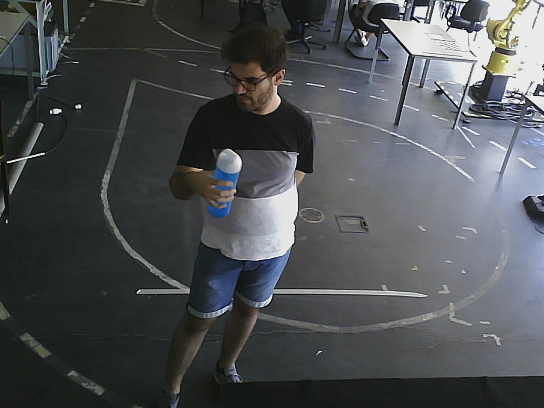
\includegraphics[width=0.49\textwidth]{figs/dataset_preprocessing1_1.png} \ 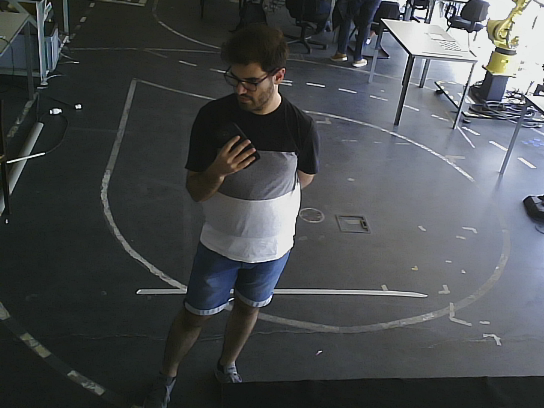
\includegraphics[width=0.49\textwidth]{figs/dataset_preprocessing1_2.png}}
    \caption{Dataset examples holding a bottle (left) and a phone (right).}
    \label{fig:dataset_examples}
\end{figure}

Naturally, the successive frames could lead to similar grasping patterns from different views. To investigate intra-user variability and to ensure robust model training, users are instructed to perform multiple grasping trials of the selected object across four distinct acquisition sessions. Bearing this in mind, the data acquisition system was designed to facilitate the fast generation of training datasets, accommodating the inclusion of new users and/or additional acquisition sessions. On the one hand, the system is integrated into the workflow of the proposed object recognition framework. On the other hand, it is particularly well-suited for implementation in industrial settings where end-users may not possess extensive expertise in machine learning or computer vision. The instructions provided to users during the data acquisition sessions were intentionally straightforward, ensuring that non-experts could readily participate in the process.

Videos over four sessions per user were recorded at 10 frames per second. For each object and each user, four data acquisition sessions were carried out, which gave rise to the dataset used in the study. Therefore, the dataset consists of a total of \num{11054} samples, distributed practically equally across the three participants (around \num{3600} samples per participant) and the four objects (between \num{2618} and \num{2849} samples per object). The exact number of samples of the entire dataset per class and per user is shown in \autoref{tab:dataset}.

\begin{table}[ht] 
\centering
\caption{Number of samples in the dataset per class and user}
\label{tab:dataset}
\begin{tabular}{lccccc}
\toprule
Dataset & Bottle & Cube & Phone & Screwdriver & Total \\
\midrule
User1 & \num{828} & \num{928} & \num{950} & \num{957} & \num{3663}\\
User2 & \num{886} & \num{926} & \num{939} & \num{946} & \num{3697}\\
User3 & \num{904} & \num{907} & \num{937} & \num{946} & \num{3694}\\
\midrule
Total & \num{2618} & \num{2761} & \num{2826} & \num{2849} & \num{11054}\\
\bottomrule
\end{tabular}
\end{table}

\subsection{Preprocessing}

After having a dataset, the data had to be processed to have a fitting structure to be used in the model training. The images from the videos were processed using the Mediapipe hands model resulting in 21 points for each hand detected (\autoref{fig:dataset_examples2}).

\begin{figure}[ht]
    \centerline{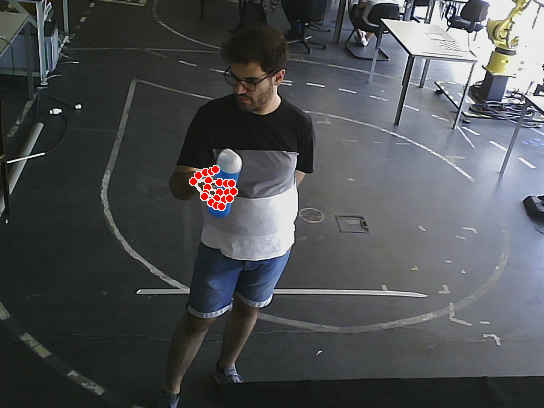
\includegraphics[width=0.49\textwidth]{figs/dataset_preprocessing2_1.png} \ 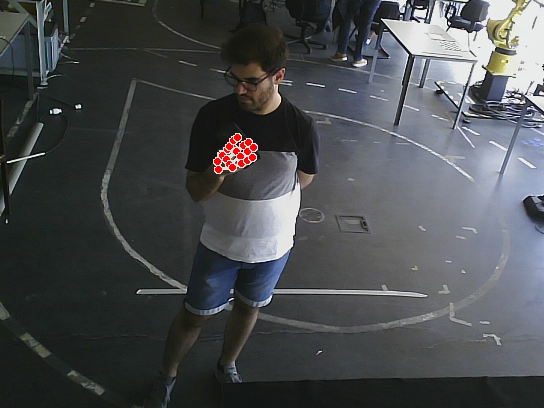
\includegraphics[width=0.49\textwidth]{figs/dataset_preprocessing2_2.png}}
    \caption{Points detected on the pictures in \autoref{fig:dataset_examples} by Mediapipe Hands Model.}
    \label{fig:dataset_examples2}
\end{figure}

The points corresponding to the right hand are then subject to further transformations and normalization. First, the original coordinates of the keypoints (raw data), which are already normalized within the range of 0 to 1 are converted into coordinates relative to a reference. Specifically, for each keypoint $P = (x,y,z)$, the coordinates of the reference point are subtracted $P_{ref} = (x_{ref}, y_{ref}, z_{ref})$ from them to obtain relative coordinates $P_{rel} = (x_{rel}, y_{rel}, z_{rel})$. In this study, the reference is defined as the centroid $C$ of the set of hand keypoints %\cred{[So $C=P_{ref}$?YES!]}. 
This transformation into relative coordinates is particularly useful because the absolute position of the hands in the image may vary from frame to frame due to different distances from the camera or hand orientations. Instead, relative coordinates are translation invariant and they reduce the influence of any rotations that might be present in the raw data. Therefore, the network will focus on the spatial relationships between keypoints, rather than their absolute positions, making it less sensitive to hand orientations and scale variations.

After obtaining the relative coordinates with respect to the reference point, scaling is applied to each dimension independently by dividing by an appropriate constant to ensure that the hand’s representation spans the entire range, as follows:
\begin{equation}
scaleFactor = \frac {0.5}{\max(\{\lvert x_i \rvert,\lvert y_i \rvert,\lvert z_i\rvert\}: i=1,\cdots,n)} \text{  ,}
\end{equation}
%
where $\{x_i,y_i,z_i\}$ denote relative coordinates. This feature scaling revealed to be a valuable pre-processing step to help make the data more consistent, helping the model to learn the relevant patterns without being influenced by variations in hand position, hand size, or scale. Further, it helps to maximize the separation among keypoints, helping the model to discriminate the output class. Finally, a uniform adjustment is made by adding 0.5 to each coordinate, centering the points between 0 and 1 on the scale. It is important to note that throughout the point processing, the order of the points is never changed, and therefore the models can take advantage of this structure. \autoref{fig:dataset_examples3} shows examples of the normalized keypoints representation expressed according to the previous steps, that is: 
\begin{equation}
P_{norm} = (P - C) \times scaleFactor + 0.5\text{ .}
\end{equation}

\begin{figure}[ht]
    \centerline{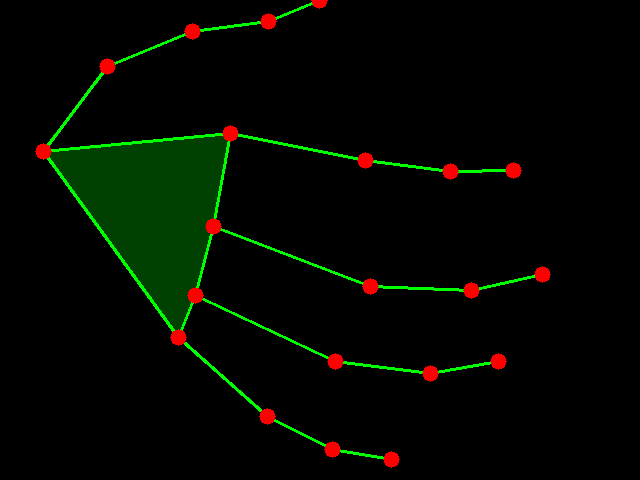
\includegraphics[width=0.49\textwidth]{figs/dataset_preprocessing3_1.png} \ 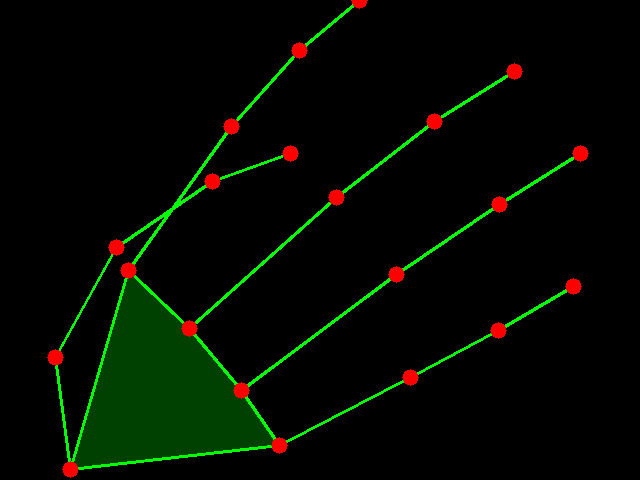
\includegraphics[width=0.49\textwidth]{figs/dataset_preprocessing3_2.png}}
    \caption{Points from the pictures in \autoref{fig:dataset_examples2} after normalization.}
    \label{fig:dataset_examples3}
\end{figure}

\subsection{Train-Validation-Test Split}

In order to train the model, the entire dataset is initially split into training and test sets using an indicative 80-20 ratio (the exact ratio can vary slightly depending on the experiment). Subsequently, the training set is further divided into a training subset and a validation subset using the same ratio. Additionally, early stopping was set up so that the model would stop training after 200 epochs without a better validation loss and restore the best weights. During hyperparameter optimization, the different combinations are tested using 4-fold cross-validation, which means that the model is trained four times, and therefore every sample of data in the initial training and validation set was used both for training and validation.

\section{K-Means Clustering}
\label{section:kmeans_clustering}

% After applying pre-processing steps to the raw data, we divided the dataset, consisting of \num{11054} samples, into training (\SI{80}{\percent}) and testing subsets (\SI{20}{\percent}).

Before describing the methodology adopted for recognizing grasping patterns, a statistical analysis was conducted on the entire dataset obtained from MediaPipe using K-means clustering. Initially, this algorithm was applied to learn the cluster structure within the training data. Subsequently, the model's performance was assessed using a separate and previously unseen test dataset.

The analysis results are visualized in a 4$\times$4 matrix, denoted as the "True Labels" vs. "Assigned Cluster" matrix (see \autoref{fig:kmeans_matrix}). This matrix provides a comprehensive view of the K-means clustering method's performance in object recognition and it enables the computation of the proportion of objects assigned to each cluster. This cluster analysis provides valuable insights into the relationships between hand poses and class labels. First, the analysis of the relationship between clusters and class labels in hand pose data reveals that certain clusters, like clusters 0 and 3, exhibit a diverse mix of all classes. Second, in the test data, cluster 0 encompasses a substantial \SI{39.8}{\percent} of the samples. Third, and of utmost importance, the K-means clustering results indicate that the clusters do not closely align with the class labels, which may indeed present challenges for the chosen classifier.

\begin{figure}[ht]
    \centering
    {\fontsize{10}{12}\selectfont\includesvg[width=0.5\textwidth]{figs/kmeans_matrix.svg}}
    \caption{The distribution of test dataset samples from each class within each cluster.}
    \label{fig:kmeans_matrix}
\end{figure}

The complexity of the problem is increased by user dependency and the variability observed within the same subject during different trials of grasping the same object. Given these challenges, a supervised learning approach, such as a \acs{cnn}, emerges as a suitable choice, as it can autonomously learn hierarchical features and patterns directly from the data, irrespective of the initial cluster structure. Deep learning models, in particular, excel in addressing the intricacies of hand posture recognition and demonstrating robust generalization across different users, effectively capturing intra-user variations, provided that the training dataset exhibits diversity and represents the target scenarios.

\section{\acl{cnn} Classifier}
\label{section:cnn_classifier}

\acfp{cnn} excel at detecting local relations, which makes them an advantageous solution for this problem given that each sample provided to the model is made of the 21 3D points that always follow the same structure representing the right hand. Although the input data is bi-dimensional (21$\times$3) resulting in a 2D kernel, a one-dimensional convolutional neural network was used so that the kernel only moves in one direction including all the point coordinates.

\subsection{Model Selection}

The backbone of the developed \acs{cnn} comprises a total of three convolutional layers each with 64 feature maps and ReLU activation functions. 
The first layer uses a kernel size of 3$\times$3 pixels performing a 1D convolution on the 3$\times$21 data with a stride of 1 pixel. The flattened output from the final layer is connected to a dense layer with 128 neurons, followed by another dense layer with the number of neurons equal to the number of classes. The output layer consists of the final connect layer with softmax activation. The softmax function takes a vector of real-valued scores (often called logits) and transforms them into a probability distribution over multiple classes. For the classification task with 4 classes, the output layer has 4 neurons, each representing the probability of the input belonging to a particular class. To prevent overfitting, dropout layers are incorporated after each fully connected layer.

To optimize the described architecture, three common hyperparameters in \acs{cnn}s were optimized to obtain even better results. These were the initial learning rate for the model training, the kernel size used by the convolutional layers, and the dropout rate. The number of convolutional layers was also tested alongside them, given that, according to manual testing, it also affected the model results without changing the number of trainable parameters. \autoref{table:cnn_hyperparameters} shows the values tested for each hyperparameter.

\begin{table}[ht]
    \centering
    \caption{Tested hyperparameter values (\acs{cnn} model)}
    \label{table:cnn_hyperparameters}
    \begin{tabular}{ll}
        \toprule
        Initial Learning Rate & 0.01, 0.001, 0.0001 \\
        Kernel Size & 2, 3 \\
        Dropout Rate & 0.0, 0.1, 0.2, 0.3, 0.4, 0.5 \\
        Number of Convolutional Layers & 1, 2, 3 \\
        \bottomrule
    \end{tabular}
\end{table}

In order to choose the best combination of these hyperparameters, all combinations were tested using 4-fold cross-validation, and the average result of each combination was obtained. The combination in \autoref{table:cnn_best_hyperparameters} resulted in the lowest average loss and an average accuracy of \SI{94.20}{\percent}.

\begin{table}[ht]
    \centering
    \caption{Best hyperparameters (\acs{cnn} model)}
    \label{table:cnn_best_hyperparameters}
    \begin{tabular}{ll}
        \toprule
        Initial Learning Rate & 0.001 \\
        Kernel Size & 3 \\
        Dropout Rate & 0.5 \\
        Number of Convolutional Layers & 2 \\
        \bottomrule
    \end{tabular}
\end{table}

The final model can be seen in \autoref{fig:cnn_architecture} and it has \num{156644} trainable parameters. It is made of two convolutional layers followed by three dense layers, with the third being the output layer. Between the convolutional and the dense layers and between both dense layers, there is also a dropout layer to help with overfitting.

\begin{figure}[ht]
    \centering
    {\fontsize{10}{12}\selectfont\includesvg[width=0.85\textwidth]{figs/cnn_architecture.svg}}
    \caption{\acs{cnn} model architecture.}
    \label{fig:cnn_architecture}
\end{figure}

\subsection{Performance Evaluation}

The final \acs{cnn} architecture was trained resulting in the learning curves in \autoref{fig:cnn_loss} and \autoref{fig:cnn_acc}. According to the figures, the best validation loss occurred around the 375th epoch, with the training stopping 200 epochs later.

\begin{figure}[ht]
    \centering
    {\fontsize{9.5}{12}\selectfont\includesvg[width=0.95\textwidth]{figs/cnn_loss_comparison.svg}}
    \caption{Training and validation loss evolution during the \acs{cnn}'s training.}
    \label{fig:cnn_loss}
\end{figure}

\begin{figure}[ht]
    \centering
    {\fontsize{9.5}{12}\selectfont\includesvg[width=0.95\textwidth]{figs/cnn_acc_comparison.svg}}
    \caption{Training and validation accuracy evolution during the \acs{cnn}'s training.}
    \label{fig:cnn_acc}
\end{figure}

After the model finished training, the metrics in the \autoref{table:cnn_dataset2_results} were obtained. Given that the test accuracy was over \SI{92}{\percent}, it can be concluded that the model managed to generalize its knowledge from the training data to classify data it has never seen before. Additionally, the confusion matrix in \autoref{fig:cnn_dataset2_confusion_matrix} shows that the screwdriver was the object the model managed to predict more accurately. This can be because the hand geometry that allows a person to intuitively grasp a screwdriver is more restricted.

\begin{table}[ht]
    \centering
    \caption{\acs{cnn} metrics}
    \label{table:cnn_dataset2_results}
    \begin{tabular}{cccc}
        \toprule
        Accuracy & Precision & Recall & F1-Score \\
        \midrule
        0.9240 & 0.9242 & 0.9240 & 0.9240 \\
        \bottomrule
    \end{tabular}
\end{table}

\begin{figure}[ht]
    \centering
    {\fontsize{10}{12}\selectfont\includesvg[width=0.4\textwidth]{figs/cnn_conf_matrix.svg}}
    \caption{\acs{cnn} confusion matrix.}
    \label{fig:cnn_dataset2_confusion_matrix}
\end{figure}

\section{Transformer Neural Network Classifier}
\label{section:transformer_classifier}

As said in \autoref{subsection:transformer_neural_networks}, Transformer Neural Networks shine at capturing long-range dependencies and relationships. Therefore, because the points obtained from Mediapipe have a specific order, this ability can be used to process structured data and effectively capture dependencies and patterns.

\subsection{Model Selection}

For this work, a Transformer architecture adapted from an example in the Keras documentation\footnote{Transformer Keras Example: \url{https://keras.io/examples/timeseries/timeseries_transformer_classification}} was tested and manually optimized. The resulting architecture can be seen in \autoref{fig:transformer_architecture} and it has \num{16384} trainable parameters. It is made of two Transformer encoder stacks (\autoref{fig:transformer_encoder_architecture}) comprised of the following layers: multi-head self-attention, layer normalization, and feedforward neural networks. Within each encoder, multi-head self-attention is applied to capture dependencies among the keypoints, where four attention heads are used for enhanced feature extraction. Following self-attention, two position-wise feedforward neural networks are employed to process the attended features and capture complex patterns. Layer normalization is applied after each sub-layer to stabilize the activations and facilitate training convergence. 

\begin{figure}[ht]
    \centering
    {\fontsize{10}{12}\selectfont\includesvg[width=0.8\textwidth]{figs/transformer_encoder.svg}}
    \caption{Transformer encoder block.}
    \label{fig:transformer_encoder_architecture}
\end{figure}

\begin{figure}[ht]
    \centering
    {\fontsize{10}{12}\selectfont\includesvg[width=0.8\textwidth]{figs/transformer_architecture.svg}}
    \caption{Transformer model architecture.}
    \label{fig:transformer_architecture}
\end{figure}

To further optimize the previous architecture, three hyperparameters were optimized to improve the performance of the model. These were the initial learning rate for the model training, the dropout rate inside each transformer block, and the dropout rate of the \acs{mlp} at the end of the model. \autoref{table:transformer_hyperparameters} shows the values tested for each hyperparameter.

\begin{table}[ht]
    \centering
    \caption{Tested hyperparameter values (Transformer model)}
    \label{table:transformer_hyperparameters}
    \begin{tabular}{ll}
        \toprule
        Initial Learning Rate & 0.01, 0.001, 0.0001 \\
        Dropout Rate & 0.0, 0.1, 0.2, 0.3, 0.4, 0.5 \\
        \acs{mlp} Dropout Rate & 0.0, 0.1, 0.2, 0.3, 0.4, 0.5 \\
        \bottomrule
    \end{tabular}
\end{table}

In order to choose the best combination of these hyperparameters, all combinations were tested using 4-fold cross-validation, and the combination with the smallest average validation loss was chosen. This combination can be seen in \autoref{table:transformer_best_hyperparameters} having an average accuracy of \SI{92.24}{\percent}.

\begin{table}[ht]
    \centering
    \caption{Best hyperparameters (Transformer model)}
    \label{table:transformer_best_hyperparameters}
    \begin{tabular}{ll}
        \toprule
        Learning Rate & 0.0001 \\
        Dropout Rate & 0.5 \\
        \acs{mlp} Dropout Rate & 0.1 \\
        \bottomrule
    \end{tabular}
\end{table}

\subsection{Performance Evaluation}

The final architecture was trained resulting in the learning curves in \autoref{fig:transformer_loss} and \autoref{fig:transformer_acc}. According to the figures, the best validation loss occurred around the 3500th epoch, with the training stopping 200 epochs later.

\begin{figure}[ht]
    \centering
    {\fontsize{9.5}{12}\selectfont\includesvg[width=0.95\textwidth]{figs/transformer_loss_comparison.svg}}
    \caption{Training and validation loss evolution during the Transformer's training.}
    \label{fig:transformer_loss}
\end{figure}

\begin{figure}[ht]
    \centering
    {\fontsize{9.5}{12}\selectfont\includesvg[width=0.95\textwidth]{figs/transformer_acc_comparison.svg}}
    \caption{Training and validation accuracy evolution during the Transformer's training.}
    \label{fig:transformer_acc}
\end{figure}

With the model training phase finished, the metrics on \autoref{table:transformer_dataset2_results} were obtained using the test set. Considering that the accuracy surpassed \SI{91}{\percent}, one can conclude that the model successfully generalized the knowledge from the training data to classify previously unseen data. Additionally, the results from the obtained confusion matrix (\autoref{fig:transformer_dataset2_confusion_matrix}) were similar to the \acs{cnn} with the screwdriver being the object predicted more accurately.

\begin{table}[ht]
    \centering
    \caption{Transformer metrics}
    \label{table:transformer_dataset2_results}
    \begin{tabular}{cccc}
        \toprule
        Accuracy & Precision & Recall & F1-Score \\
        \midrule
        0.9109 & 0.9115 & 0.9109 & 0.9109 \\
        \bottomrule
    \end{tabular}
\end{table}

\begin{figure}[ht]
    \centering
    {\fontsize{10}{12}\selectfont\includesvg[width=0.4\textwidth]{figs/transformer_conf_matrix.svg}}
    \caption{Transformer confusion matrix.}
    \label{fig:transformer_dataset2_confusion_matrix}
\end{figure}

\section{Comparative Analysis of Deep Models Generalization Ability}
\label{section:comparative_analysis}

This section provides a comparative analysis of the performance of a \acs{cnn} model against a transformer model for the recognition of the human-grasped object from the hand keypoints. Three main experiments were designed to evaluate the classification performance of the two architectures under comparison when they were fed with the same data. With the three experiments, the intent was to study the generalization capacity of the deep model in unseen data, taking into account the different users and the different data acquisition sessions.

\subsection{Experiments and Metrics}
In the context of this research on developing a hand-object recognition classifier utilizing keypoints provided by the MediaPipe Hands Model, a series of experiments was conducted to evaluate the classifier's performance comprehensively, as follows:
\begin{itemize}
  
  \item \textbf{Experiment 1: Session-Based Test}: the first experiment aims to assess the impact of session-based testing on the classifier's performance. For that purpose, the classifier will be trained on data from all users and all acquisition sessions except one that will be used for testing.
  
  \item \textbf{Experiment 2: User-Specific Test}: in the pursuit of refining the hand-object recognition classifier, a second experiment with a focus on individual user data was conducted. This experiment aims to provide insights into how the classifier performs when trained and tested on data collected from a single user, with the process repeated separately for each of the selected users.
  
  \item \textbf{Experiment 3: Leave-One-User-Out Test:}: the third experiment follows a distinctive approach termed the "Leave-One-User-Out Test". This experiment is designed to evaluate the classifier's performance when trained on data from two users and tested on data from the third user.
  
\end{itemize}

All experiments carried out take into account the intrinsic variability of performance estimation by conducting 50 Monte-Carlo simulations. Metrics such as accuracy, precision, recall, and F1-score were used to quantify the model’s effectiveness in recognizing the grasped object. Also, confusion matrices help identify specific areas where the model may excel or struggle in the classification task.

\subsection{Session-Based Testing}
In order to investigate the influence of session-based testing, the dataset was divided into two configurations. In the first configuration, referred to as the "Full Dataset" scenario, the entire dataset was employed consisting of \num{11054} samples for both training and testing. First, the dataset was randomly split into training (\num{6632} samples), validation (\num{2211} samples), and testing (\num{2211} samples) subsets. This setup aims to evaluate the classifier's performance when trained on a diverse set of hand-object interactions. \autoref{table:results_first_case} summarizes the results of evaluating the performance of the two models in the "Full Dataset" scenario in terms of accuracy, precision, recall, and F1-score. The \acs{cnn} and Transformer show similar results with robust scores around \SI{92}{\percent} and \SI{90}{\percent}, respectively. The confusion matrices in \autoref{fig:multi_user_conf_matrices} show that the classifiers excel in distinguishing between the different classes, maintaining high accuracy. However, this outcome underscores the classifier's ability to generalize across a diverse range of hand-object interactions, as it was trained on a dataset encompassing multiple users and multiple data acquisition sessions.

\begin{table}[ht]
    \centering
    \caption{"Full Dataset" performance metrics}
    \label{table:results_first_case}
    \begin{tabular}{lcccc}
        \toprule
        Model & Accuracy & Precision & Recall & F1-Score \\
        %\hline
        \midrule
        \acs{cnn} & \textbf{0.9210} & \textbf{0.9214} & \textbf{0.9211} & \textbf{0.9211} \\
        %\hline
        Transformer & 0.9017 & 0.9020 & 0.9016 & 0.9017 \\
        \bottomrule
    \end{tabular}
\end{table}

\begin{figure}[ht]
    \centering
    \begin{subfigure}[b]{0.32\columnwidth}
        {\fontsize{8}{10}\selectfont\includesvg[width=\textwidth]{figs/conv_1d_multi_user_conf_matrix.svg}}
        \caption{\centering}
        % \label{}
    \end{subfigure} \
    \begin{subfigure}[b]{0.32\columnwidth}
        {\fontsize{8}{10}\selectfont\includesvg[width=\textwidth]{figs/transformer_multi_user_conf_matrix.svg}}
        \caption{\centering}
        % \label{}
    \end{subfigure}
    \caption[Multi-User Confusion matrices]{"Full Dataset" confusion matrices: (a) \acs{cnn} model, (b) Transformer model.}
    \label{fig:multi_user_conf_matrices}
\end{figure}

In the second configuration, one session was isolated from each user for testing (\num{2731} samples), while the remaining sessions from all users were used for training (\num{8289} samples). The aim was to determine how the inclusion of session-specific data impacts the classifier performance. The results depicted in \autoref{table:results_first_caseB} show the discrepancy in classifier accuracy between the "Full Dataset" and the "Session-Based Testing" scenarios. Further, the confusion matrix in \autoref{fig:cnn_multi_user_by_session_conf_matrices} compares the actual target with those predicted by the \acs{cnn} model. The classifier is making accurate and correct predictions for the majority of classes, while struggling to recognize accurately examples belonging to specific classes, such as the "phone" in the third data acquisition session (the same with the Transformer).

\begin{table}[ht]
    \captionsetup{width=0.8\textwidth}
    \centering
    \caption{"Session-Based Testing" performance metrics where data from each session only appears in one set. For example, the "Session 1" column means that data from that session of all users is used in testing, while the remaining sessions are used for training.}
    \label{table:results_first_caseB}
    \begin{tabular}{l|lcccc}
        \toprule
        Metric & Model & Session 1 & Session 2 & Session 3 & Session 4 \\
        \midrule
        \multirow{2}{*}{Accuracy} & \acs{cnn} & \textbf{0.8493} & \textbf{0.8138} & 0.7844 & \textbf{0.7718} \\
        %\cline{2-6}
        & Transformer & 0.8458 & 0.8027 & \textbf{0.7902} & 0.7613 \\
        \midrule
        \multirow{2}{*}{Precision} & \acs{cnn} & \textbf{0.8515} & \textbf{0.8160} & 0.8024 & \textbf{0.7723} \\
        %\cline{2-6}
        & Transformer & 0.8469 & 0.8028 & \textbf{0.8045} & 0.7623 \\
        \midrule
        \multirow{2}{*}{Recall} & \acs{cnn} & \textbf{0.8493} & \textbf{0.8138} & 0.7844 & \textbf{0.7718} \\
        %\cline{2-6}
        & Transformer & 0.8458 & 0.8027 & \textbf{0.7902} & 0.7613 \\
        \midrule
        \multirow{2}{*}{F1-Score} & \acs{cnn} & \textbf{0.8499} & \textbf{0.8136} & 0.7878 & \textbf{0.7717} \\
        %\cline{2-6}
        & Transformer & 0.8461 & 0.8019 & \textbf{0.7932} & 0.7614 \\
        \bottomrule
    \end{tabular}
\end{table}

\begin{figure}[ht]
    \centering
    \begin{subfigure}[b]{0.32\columnwidth}
        {\fontsize{8}{10}\selectfont\includesvg[width=\textwidth]{figs/conv_1d_multi_user_by_session_session_1_conf_matrix.svg}}
        \caption{\centering}
        % \label{}
    \end{subfigure} \ \
    \begin{subfigure}[b]{0.32\columnwidth}
        {\fontsize{8}{10}\selectfont\includesvg[width=\textwidth]{figs/conv_1d_multi_user_by_session_session_2_conf_matrix.svg}}
        \caption{\centering}
        % \label{}
    \end{subfigure}
    \par\medskip
    \begin{subfigure}[b]{0.32\columnwidth}
        {\fontsize{8}{10}\selectfont\includesvg[width=\textwidth]{figs/conv_1d_multi_user_by_session_session_3_conf_matrix.svg}}
        \caption{\centering}
        % \label{}
    \end{subfigure} \ \
    \begin{subfigure}[b]{0.32\columnwidth}
        {\fontsize{8}{10}\selectfont\includesvg[width=\textwidth]{figs/conv_1d_multi_user_by_session_session_4_conf_matrix.svg}}
        \caption{\centering}
        % \label{}
    \end{subfigure}
    \caption{"Session-Based Testing" confusion matrices (\acs{cnn} model): session 1 (a) to session 4 (d).}
    \label{fig:cnn_multi_user_by_session_conf_matrices}
\end{figure}

%\begin{figure}[!ht]
%    \centering
%    \begin{subfigure}[b]{0.32\columnwidth}
%        {\fontsize{8}{10}\selectfont\includesvg[width=\textwidth]{figs/transformer_multi_user_session_1_conf_matrix.svg}}
%        \caption{\centering}
        % \label{}
%    \end{subfigure} \ \
 %   \begin{subfigure}[b]{0.32\columnwidth}
 %       {\fontsize{8}{10}\selectfont\includesvg[width=\textwidth]{figs/transformer_multi_user_session_2_conf_matrix.svg}}
 %       \caption{\centering}
 %       % \label{}
 %   \end{subfigure}
 %   \par\medskip
 %   \begin{subfigure}[b]{0.32\columnwidth}
 %       {\fontsize{8}{10}\selectfont\includesvg[width=\textwidth]{figs/transformer_multi_user_session_3_conf_matrix.svg}}
 %       \caption{\centering}
 %       % \label{}
 %   \end{subfigure} \ \
 %   \begin{subfigure}[b]{0.32\columnwidth}
 %       {\fontsize{8}{10}\selectfont\includesvg[width=\textwidth]{figs/transformer_multi_user_session_4_conf_matrix.svg}}
 %       \caption{\centering}
 %       % \label{}
 %   \end{subfigure}
 %   \caption[Transformer Multi-User Confusion matrices (with attention to sessions)]{Transformer Multi-User Confusion matrices (with attention to sessions)}
 %   \label{fig:transformer_multi_user_by_session_conf_matrices}
%\end{figure}

\subsection{User-Specific Test}

The experiment described in this subsection focuses on the variability in hand configurations and keypoint patterns for the same user over time (i.e., under different conditions imposed by the four data acquisition sessions carried out). Once again, two distinct dataset configurations were constructed for each user. In the first configuration ("Full User Dataset"), the entire dataset for a single user was used, with the process repeated separately for all others. This simulates a scenario where the classifier is trained and tested on all available data for a single user based on a random split using an 80-20 ratio. The performance of the \acs{cnn} and transformer models in the "Full User Dataset" scenario is summarized in \autoref{table:results_second_case}. The \acs{cnn} presents slightly better results than the transformer in different metrics, while User1's performance stands out. The confusion matrices show that the classifiers excel in distinguishing between the different classes with high accuracy (see \autoref{fig:conf_matrix_full_user} relating to the \acs{cnn} model). 

\begin{table}[ht]
    \centering
    \caption{"Full User Dataset" performance metrics.}
    \label{table:results_second_case}
    \begin{tabular}{l|lccc}
        \toprule
        Metric & Model & User1 & User2 & User3 \\
        \midrule
        \multirow{2}{*}{Accuracy} & \acs{cnn} & \textbf{0.9674} & \textbf{0.9100} & \textbf{0.9163} \\
        & Transformer & 0.9423 & 0.8929 & 0.8730 \\
        \midrule
        \multirow{2}{*}{Precision} & \acs{cnn} & \textbf{0.9678} & \textbf{0.9109} & \textbf{0.9171} \\
        & Transformer & 0.9435 & 0.8943 & 0.8745 \\
        \midrule
        \multirow{2}{*}{Recall} & \acs{cnn} & \textbf{0.9674} & \textbf{0.9100} & \textbf{0.9163} \\
        & Transformer & 0.9423 & 0.8929 & 0.8730 \\
        \midrule
        \multirow{2}{*}{F1-Score} & \acs{cnn} & \textbf{0.9675} & \textbf{0.9101} & \textbf{0.9164} \\
        & Transformer & 0.9423 & 0.8930 & 0.8729 \\
        \bottomrule
    \end{tabular}
\end{table}

\begin{figure}[ht]
    \centering
    \begin{subfigure}[b]{0.32\columnwidth}
        {\fontsize{8}{10}\selectfont\includesvg[width=\textwidth]{figs/conv_1d_intra_user_joel_conf_matrix.svg}}
        \caption{\centering}
        % \label{}
    \end{subfigure} \
    \begin{subfigure}[b]{0.32\columnwidth}
        {\fontsize{8}{10}\selectfont\includesvg[width=\textwidth]{figs/conv_1d_intra_user_manuel_conf_matrix.svg}}
        \caption{\centering}
        % \label{}
    \end{subfigure} \
    \begin{subfigure}[b]{0.32\columnwidth}
        {\fontsize{8}{10}\selectfont\includesvg[width=\textwidth]{figs/conv_1d_intra_user_pedro_conf_matrix.svg}}
        \caption{\centering}
        % \label{}
    \end{subfigure}
    \caption{"Full User Dataset" confusion matrices (\acs{cnn} model): (a) User1, (b) User2, and (c) User3.}
    \label{fig:conf_matrix_full_user}
\end{figure}

%\begin{figure}[H]
%    \centering
%    \begin{subfigure}[b]{0.32\columnwidth}
%        {\fontsize{8}{10}\selectfont\includesvg[width=\textwidth]{figs/transformer_intra_user_joel_conf_matrix.svg}}
%        \caption{\centering}
%        % \label{}
%    \end{subfigure} \
%    \begin{subfigure}[b]{0.32\columnwidth}
%        {\fontsize{8}{10}\selectfont\includesvg[width=\textwidth]{figs/transformer_intra_user_manuel_conf_matrix.svg}}
%        \caption{\centering}
%        % \label{}
%    \end{subfigure} \
%    \begin{subfigure}[b]{0.32\columnwidth}
%        {\fontsize{8}{10}\selectfont\includesvg[width=\textwidth]{figs/transformer_intra_user_pedro_conf_matrix.svg}}
%        \caption{\centering}
%        % \label{}
%    \end{subfigure}
%    \caption[Transformer Intra-User Confusion matrices]{Transformer Intra-User Confusion matrices}
    \label{fig:conf_matrix_examplesC}
%\end{figure}

In the second configuration, the data of one acquisition session for a specific user was isolated, dedicating it exclusively to the testing phase. Meanwhile, the remaining sessions' data from the same user were employed for training. This "Session-Based User Testing" setup mirrors scenarios where a classifier must adapt to recognize objects manipulated by a user based on a limited history of interactions. The results in \autoref{table:results_session_based_user1}, relating to User1, reveal interesting insights into the classifier's adaptability within the context of different user behaviors across multiple sessions. First, varying levels in all metrics across sessions with a range between \SI{78.8}{\percent} and \SI{92.6}{\percent} can be observed. The decrease in the evaluation metrics between the "Full User Dataset" and "Session-Based User Testing" scenarios highlights the importance of user-specific adaptation. The confusion matrices (see \autoref{fig:Session_Based_User1_Testing_CNN}) also reveal lower performances in certain classes, but these vary from session to session. These results emphasize the importance of considering session-specific variations and user behaviors when training and evaluating the classifier. 

\begin{table}[ht]
    \captionsetup{width=0.8\textwidth}
    \centering
    \caption{"Session-Based User1 Testing" performance metrics (each column indicates the specific session used in testing the model).}
    \label{table:results_session_based_user1}
    \begin{tabular}{l|lcccc}
        \toprule
        Metric & Model & Session 1 & Session 2 & Session 3 & Session 4 \\
        \midrule
        \multirow{2}{*}{Accuracy} & \acs{cnn} & \textbf{0.9257} & \textbf{0.8364} & \textbf{0.9053} & \textbf{0.7883} \\
        & Transformer & 0.9078 & 0.8171 & 0.8742 & 0.7636 \\
        \midrule
        \multirow{2}{*}{Precision} & \acs{cnn} & \textbf{0.9288} & \textbf{0.8543} & \textbf{0.9135} & \textbf{0.7971} \\
        & Transformer & 0.9112 & 0.8401 & 0.8806 & 0.7846 \\
        \midrule
        \multirow{2}{*}{Recall} & \acs{cnn} & \textbf{0.9257} & \textbf{0.8364} & \textbf{0.9053} & \textbf{0.7884} \\
        & Transformer & 0.9078 & 0.8172 & 0.8742 & 0.7636 \\
        \midrule
        \multirow{2}{*}{F1-Score} & \acs{cnn} & \textbf{0.9261} & \textbf{0.8382} & \textbf{0.9073} & \textbf{0.7892} \\
        & Transformer & 0.9083 & 0.8196 & 0.8759 & 0.7671 \\
        \bottomrule
    \end{tabular}
\end{table}

\begin{figure}[ht]
    \centering
    \begin{subfigure}[b]{0.32\columnwidth}
        {\fontsize{8}{10}\selectfont\includesvg[width=\textwidth]{figs/conv_1d_intra_user_by_session_joel_session_1_conf_matrix.svg}}
        \caption{\centering}
        % \label{}
    \end{subfigure} \ \
    \begin{subfigure}[b]{0.32\columnwidth}
        {\fontsize{8}{10}\selectfont\includesvg[width=\textwidth]{figs/conv_1d_intra_user_by_session_joel_session_2_conf_matrix.svg}}
        \caption{\centering}
        % \label{}
    \end{subfigure}
    \par\medskip
    \begin{subfigure}[b]{0.32\columnwidth}
        {\fontsize{8}{10}\selectfont\includesvg[width=\textwidth]{figs/conv_1d_intra_user_by_session_joel_session_3_conf_matrix.svg}}
        \caption{\centering}
        % \label{}
    \end{subfigure} \ \
    \begin{subfigure}[b]{0.32\columnwidth}
        {\fontsize{8}{10}\selectfont\includesvg[width=\textwidth]{figs/conv_1d_intra_user_by_session_joel_session_4_conf_matrix.svg}}
        \caption{\centering}
        % \label{}
    \end{subfigure}
    \caption{"Session-Based User1 Testing" confusion matrices (\acs{cnn} model).}
    \label{fig:Session_Based_User1_Testing_CNN}
\end{figure}

%\begin{figure}[!ht]
%    \centering
%    \begin{subfigure}[b]{0.32\columnwidth}
%        {\fontsize{8}{10}\selectfont\includesvg[width=\textwidth]{figs/transformer_intra_user_by_session_joel_session_1_conf_matrix.svg}}
%        \caption{\centering}
%        % \label{}
%    \end{subfigure} \ \
%    \begin{subfigure}[b]{0.32\columnwidth}
%        {\fontsize{8}{10}\selectfont\includesvg[width=\textwidth]{figs/transformer_intra_user_by_session_joel_session_2_conf_matrix.svg}}
%        \caption{\centering}
%        % \label{}
%    \end{subfigure}
%    \par\medskip
%    \begin{subfigure}[b]{0.32\columnwidth}
%        {\fontsize{8}{10}\selectfont\includesvg[width=\textwidth]{figs/transformer_intra_user_by_session_joel_session_3_conf_matrix.svg}}
%        \caption{\centering}
%        % \label{}
%    \end{subfigure} \ \
%    \begin{subfigure}[b]{0.32\columnwidth}
%        {\fontsize{8}{10}\selectfont\includesvg[width=\textwidth]{figs/transformer_intra_user_by_session_joel_session_4_conf_matrix.svg}}
%        \caption{\centering}
%        % \label{}
%    \end{subfigure}
%    \caption[Transformer Intra-User User1 Confusion matrices (with attention to sessions)]{Transformer Intra-User User1 Confusion matrices (with attention to sessions)}
%    \label{fig:transformer_multi_user_by_session_conf_matricesB}
%\end{figure}

\subsection{Leave-One-User-Out Test}
The third experiment follows a distinctive approach termed the "Leave-One-User-Out Test". This is particularly relevant in scenarios where the data is collected from multiple users (i.e., dealing with user-dependent data), and the goal is to evaluate the model's generalization ability to new individuals who were not part of the training data. In this case, the process involves training the model on data from all users except one (the user to be left out) and then evaluating the model's performance on the data from the left-out user. This experiment allows the observation of a trend and it showcases the challenges of generalization to unseen users. In order to identify the trend, the process is repeated for each user, training the model on all users except the one being evaluated. This approach ensures that each user's data is used once as a test set (around 3660 samples), while the remaining data is employed for training (around 7350 samples).

\autoref{table:results_third_case} and \autoref{fig:conf_matrix_examplesC_v2} shows the results obtained considering that only one user's data (all sessions) is used in testing the model. Although the classifier recognizes to some extent objects grasped by "User1" when it has not been explicitly trained on, the lower performance for "User2" and "User3" indicates limitations in generalization to users with distinct grasping patterns. The results indicate the difficulties the deep model faces when adapting to a new user in the absence of a dedicated training period. This emphasizes the need for personalized models or strategies that can adapt to individual user behaviors. In real-world scenarios, users may exhibit diverse hand-object interaction patterns and models should be capable of accommodating these variations. Whatever strategy is adopted, ensuring diverse and representative data (e.g., a bigger dataset) will be crucial for improving the results, either using a convolutional network as a transformer. 

\begin{table}[ht]
    \captionsetup{width=0.6\textwidth}
    \centering
    \caption{"Leave-One-User-Out Test" performance metrics where data from each user only appears in the test set. For example, the "User1" column means that data from that user is used in testing, while the data from the remaining users is used for training."}
    \label{table:results_third_case}
    \begin{tabular}{l|lccc}
        \toprule
        Metric & Model & User1 & User2 & User3 \\
        \midrule
        \multirow{2}{*}{Accuracy} & \acs{cnn} & 0.7969 & \textbf{0.5827} & \textbf{0.5488} \\
        & Transformer & \textbf{0.8006} & 0.5730 & 0.5350 \\
        \midrule
        \multirow{2}{*}{Precision} & \acs{cnn} & \textbf{0.8123} & \textbf{0.5889} & \textbf{0.5675} \\
        & Transformer & 0.8094 & 0.5794 & 0.5492 \\
        \midrule
        \multirow{2}{*}{Recall} & \acs{cnn} & 0.7969 & \textbf{0.5827} & \textbf{0.5488} \\
        & Transformer & \textbf{0.8006} & 0.5730 & 0.5350 \\
        \midrule
        \multirow{2}{*}{F1-Score} & \acs{cnn} & 0.8008 & \textbf{0.5791} & \textbf{0.5483} \\
        & Transformer & \textbf{0.8028} & 0.5702 & 0.5321 \\
        \bottomrule
    \end{tabular}
\end{table}

\begin{figure}[ht]
   \centering
   \begin{subfigure}[b]{0.32\columnwidth}
       {\fontsize{8}{10}\selectfont\includesvg[width=\textwidth]{figs/conv_1d_inter_user_joel_conf_matrix.svg}}
       \caption{\centering}
       % \label{}
   \end{subfigure} \
   \begin{subfigure}[b]{0.32\columnwidth}
       {\fontsize{8}{10}\selectfont\includesvg[width=\textwidth]{figs/conv_1d_inter_user_manuel_conf_matrix.svg}}
       \caption{\centering}
       % \label{}
   \end{subfigure} \
   \begin{subfigure}[b]{0.32\columnwidth}
       {\fontsize{8}{10}\selectfont\includesvg[width=\textwidth]{figs/conv_1d_inter_user_pedro_conf_matrix.svg}}
       \caption{\centering}
       % \label{}
   \end{subfigure}
   \caption{"Leave-One-User-Out Test" confusion matrices (\acs{cnn} model).}
   \label{fig:conf_matrix_examplesC_v2}
\end{figure}

%\begin{figure}[H]
%    \centering
%    \begin{subfigure}[b]{0.32\columnwidth}
%        {\fontsize{8}{10}\selectfont\includesvg[width=\textwidth]{figs/transformer_inter_user_joel_conf_matrix.svg}}
%        \caption{\centering}
%        % \label{}
%    \end{subfigure} \
%    \begin{subfigure}[b]{0.32\columnwidth}
%        {\fontsize{8}{10}\selectfont\includesvg[width=\textwidth]{figs/transformer_inter_user_manuel_conf_matrix.svg}}
%        \caption{\centering}
%        % \label{}
%    \end{subfigure} \
%    \begin{subfigure}[b]{0.32\columnwidth}
%        {\fontsize{8}{10}\selectfont\includesvg[width=\textwidth]{figs/transformer_inter_user_pedro_conf_matrix.svg}}
%        \caption{\centering}
%        % \label{}
%    \end{subfigure}
%    \caption[Transformer Inter-User Confusion matrices]{Transformer Inter-User Confusion matrices}
%    \label{fig:conf_matrix_examplesC_v3}
%\end{figure}

\section{Human Intention Prediction in Shared Tasks}
\label{section:human_intention_prediction}

After detailing all the processes related to the models' creation and validation, this section will cover how they can be integrated into a real-time application. In the proposed implementation, the MediaPipe Hands and Pose models have a corresponding \acs{ros} node that communicates with the others using actions. This communication method ensures that the models can run in parallel with each other and that the node that makes the requests does not need to wait for the results of the first model to make a request to the second as would be the case if services were used. Although communicating using publish/subscribe nodes would also respect the previous requirements, using actions also has the advantage of guaranteeing that the images analyzed by both models are the same. This process is managed by the Right Hand Keypoints Detection node which sends the images to the MediaPipe nodes, associates their outputs, and publishes only the right hand keypoints. The Points Normalization node is responsible for applying the remaining preprocessing steps and then publishing the normalized right-hand keypoints. Finally, the Model Prediction node contains a model trained in this work and predicts the grasped object. \autoref{fig:ml_pipeline} shows the developed implementation in \acs{ros} of data preprocessing and model prediction.

\begin{figure}[ht]
    \centering
    \begin{tikzpicture}[>=latex']
    \tikzset{block/.style= {draw, rectangle, align=center,minimum width=1.5cm,minimum height=1.5cm},
    rblock/.style={draw, shape=rectangle,rounded corners=1.5em,align=center,minimum width=2cm,minimum height=1cm},
    input/.style={ % requires library shapes.geometric
    draw,
    trapezium,
    trapezium left angle=60,
    trapezium right angle=120,
    minimum width=2cm,
    align=center,
    minimum height=1cm
    },
    }
    
    \node [rblock] (camera) {Camera\\Image};
    \node [block, above =1cm of camera] (hands_keypoints) {Mediapipe\\Hands Model};
    \node [block, below =1cm of camera] (body_keypoints) {Mediapipe\\Pose Model};
    \node [block, right =0.5cm of camera] (right_hand_keypoints_detection) {Right Hand\\Keypoints\\Detection};
    \node [block, right =2cm of right_hand_keypoints_detection] (normalization) {Points\\Normalization};
    \node [block, right =2cm of normalization] (model) {Model\\Prediction};
    \node [rblock, right =0.25cm of model] (output) {Predicted\\Object};
    %\node [below left =0.1cm of normalization] (image1) {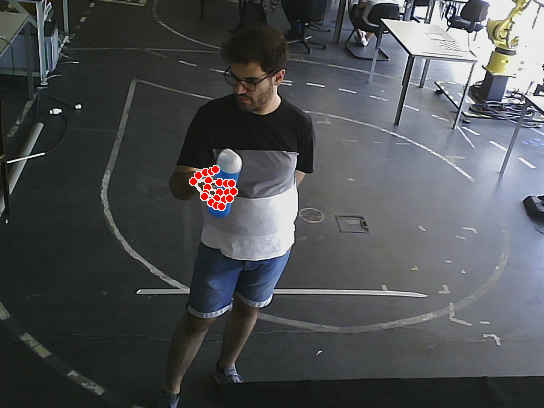
\includegraphics[width=.15\textwidth]{figs/dataset_preprocessing2_1.png}};
    %\node [below left =0.1cm of model] (image2) {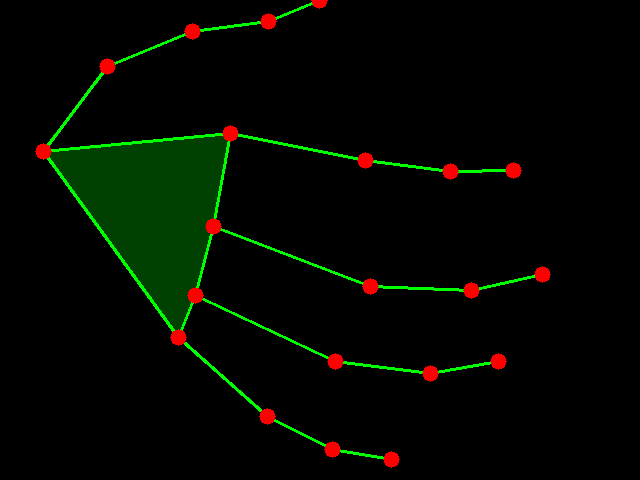
\includegraphics[width=.15\textwidth]{figs/dataset_preprocessing3_1.png}};

    \path[draw,->, text width=2cm, align=center]
                (camera) edge (hands_keypoints)
                (camera) edge (body_keypoints)
                (hands_keypoints) edge node[right, near start] {Hands\\Keypoints} (right_hand_keypoints_detection)
                (body_keypoints) edge node[right, near start] {Pose\\Keypoints} (right_hand_keypoints_detection)
                (right_hand_keypoints_detection) edge node[below] {\adjincludegraphics[width=.9\textwidth, trim={{.25\width} {0.25\height} {.25\width} {0.25\height}}, clip]{figs/dataset_preprocessing2_1.png}} (normalization)
                (normalization) edge node[below] {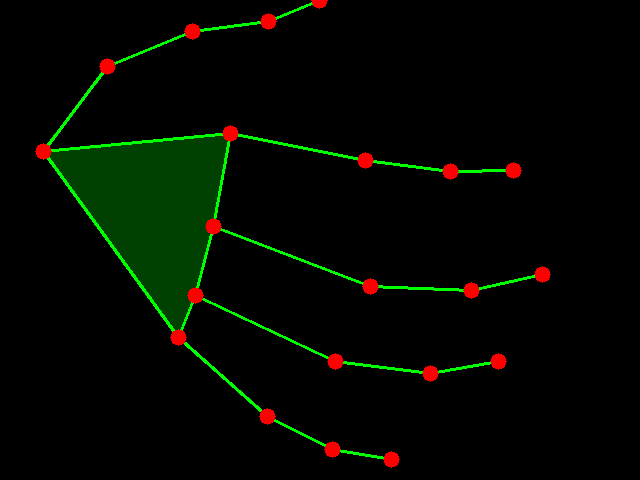
\includegraphics[width=.9\textwidth]{figs/dataset_preprocessing3_1.png}} (model)
                (model) edge (output)
                ;

    %% paths
    \if{0}
    \path[draw,->, text width=3cm, align=center]
                (camera) edge (hands_keypoints)
                (camera) edge[bend right] (body_keypoints)
                (hands_keypoints) edge node[above] {{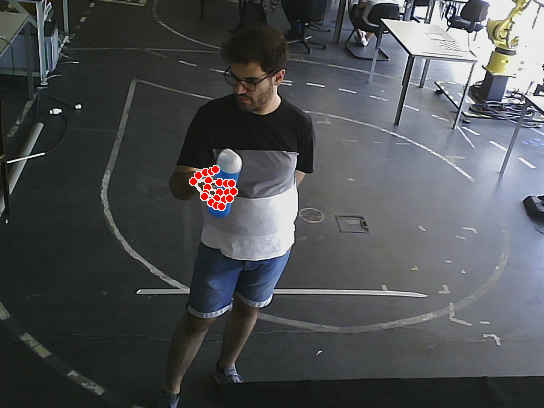
\includegraphics[width=.9\textwidth]{figs/dataset_preprocessing2_1.png}}} (body_keypoints)
                (body_keypoints) edge node[right] {right hand keypoints} (normalization) 
                (normalization) edge node[above] {normalized right hand keypoints} (model)
                (model) edge (output)
                ;
    \fi

    \if{0}
    \node [rblock] (camera) {Camera\\Image};
    \node [block, right =0.5cm of camera] (hands_keypoints) {Mediapipe\\Hands\\Model};
    \node [block, right =0.5cm of hands_keypoints] (body_keypoints) {Mediapipe\\Full Body\\Model};
    \node [block, right =0.5cm of body_keypoints] (normalization) {Points\\Normalization};
    \node [block, right =0.5cm of normalization] (model) {Model\\Prediction};
    \node [rblock, right =0.5cm of model] (output) {Predicted\\Object};

    %% paths
    \path[draw,->, text width=1.7cm, align=center]
                (camera) edge (hands_keypoints)
                (camera) edge[bend right] (body_keypoints)
                (hands_keypoints) edge (body_keypoints)
                (body_keypoints) edge (normalization) 
                (normalization) edge (model)
                (model) edge (output)
                ;
    \fi
    
\end{tikzpicture}
    \caption{\acs{ros} nodes in the object recognition pipeline.}
    \label{fig:ml_pipeline}
\end{figure}

% Given that the system processes a continuous video stream, it can generate multiple predictions per second, which can be combined to make a final decision. This approach could give priority to the most frequent label to prevent a single incorrect prediction from negatively affecting the robot's actions.

In a real-time implementation, additional processing could be made. For example, given that the system processes a continuous video stream, it can generate multiple predictions per second, which can be combined to make a final decision. This approach could give priority to the most frequent label to prevent a single incorrect prediction from negatively affecting the robot's actions. However, certain limitations would also need to be addressed. One example is how to deal with frames where the user is not holding an object. To solve this, the system could, for instance, have a threshold on the model's output probabilities to know if the hand is in fact holding an object. Another example is how to deal with occlusions given that the object can occlude the hand enough that MediaPipe stops detecting it. This could be solved using object recognition models that directly classify the object from the images or by adding more cameras. The information about which object is being grasped can then be used to make a decision. Although it was not implemented, a possible solution would be to add a new rule to the rule-based controller described in \autoref{subsection:first_anticipation_experiments}.

\section{Final Remarks}
\label{section:learning_final_remarks}

The experiments carried out provide valuable insights into the classifier's performance in different testing scenarios, especially for real-world applications. The results of the "User-Specific Test" show that the classifier's performance is influenced by the variability in interaction patterns across different sessions. This emphasizes the importance of considering session-specific variations when training and evaluating the classifier in user-centric applications (e.g., single-operator workstations). The lower accuracy in certain sessions and classes suggests the need for model refinements to deal with changes in data distribution between different work sessions. Pre-training a model on a large and diverse dataset and then fine-tuning it using data from a new session can be effective. Likewise, monitoring the model's performance in real-time and periodically retraining it with new and diverse data can help the model adapt to changing conditions and variations in different work sessions.

In dynamic settings where multiple users may interact with objects differently across multiple sessions, it is crucial for the classifier to adapt and maintain performance. The declining trend observed in the "Session-Based Testing" scenario suggests that the classifier may have difficulties in recognizing grasping patterns effectively when faced with new sessions that deviate from those in training. Once again, these results highlight the importance of considering session-specific variations when acquiring the dataset. From the perspective of model development in practical applications, the findings of this experiment emphasize the need for ongoing model refinements and adaptation strategies. Techniques such as session-specific fine-tuning or the incorporation of session-related features may prove valuable in enhancing the classifier's performance in real-world, dynamic environments.

The findings from the "Leave-One-User-Out Test" highlight the importance of personalized modeling approaches to account for user-specific patterns in the hand-object recognition system. In order to enhance the classifier's performance, it may be necessary to consider user-specific fine-tuning that can help the model better capture the nuances of new users. This personalized training can lead to better convergence and performance. This reflects the importance of actively collecting data from new users in a systematic way to adapt the model. In line with this, the implementation of a system that allows for continuous model updating as new user data becomes available can be foreseen, i.e., the model can adapt and improve over time.

In the previous tests, the training times for both architectures were recorded, which are displayed in \autoref{table:training_times}. The results consistently showed that the Transformer required approximately ten times more training time compared to the \acs{cnn}. This is due to the fact that the \acs{cnn} is a relatively simpler architecture even if the number of parameters is significantly higher in the \acs{cnn} (\num{156644} compared to \num{16384}). This information in relevant in a real-time implementation where the training time can be a deciding factor.

\begin{table}[ht]
    \centering
    \caption{Average training times comparison}
    \label{table:training_times}
    \begin{tabular}{lcc}
        \toprule
        Test & \acs{cnn} & Transformer \\
        \midrule
        Full Dataset & \SI{126.85}{\second} & \SI{1350.53}{\second} \\
        Session-Based & \SI{119.25}{\second} & \SI{1323.65}{\second} \\
        Full User Dataset & \SI{41.73}{\second} & \SI{625.90}{\second} \\
        Session-Based User1 & \SI{42.96}{\second} & \SI{517.36}{\second} \\
        Leave-One-User-Out & \SI{96.53}{\second} & \SI{995.17}{\second} \\
        \bottomrule
    \end{tabular}
\end{table}